% Figure source. `npm run notes -- build stat497` compiles it to the PDF the
% notes include and to time-state.svg for the web page. The handwritten 2 x 2
% table: whether time is discrete or continuous, against whether the values
% (the state) are. The sketches are illustrative, not data.
\documentclass[tikz,border=4pt]{standalone}
\usepackage{libertinus}
\usepackage{libertinust1math}
\definecolor{accent}{HTML}{1D4E89}
\definecolor{caution}{HTML}{9B2C2C}
\definecolor{quiet}{HTML}{6B7280}
\definecolor{hair}{HTML}{D5D9DF}

% A small pair of axes, 3.5cm by 1.9cm, with the origin at (#1,#2), and the
% panel's label under it.
\newcommand{\panel}[3]{
  \draw[quiet, line width=.5pt, -latex] (#1,#2) -- ++(3.5,0) node[right, font=\footnotesize] {$t$};
  \draw[quiet, line width=.5pt, -latex] (#1,#2) -- ++(0,1.9) node[above, font=\footnotesize] {$X(t)$};
  \node[text=quiet, font=\footnotesize, anchor=north] at (#1+1.75,#2-0.2) {#3};
}

\begin{document}
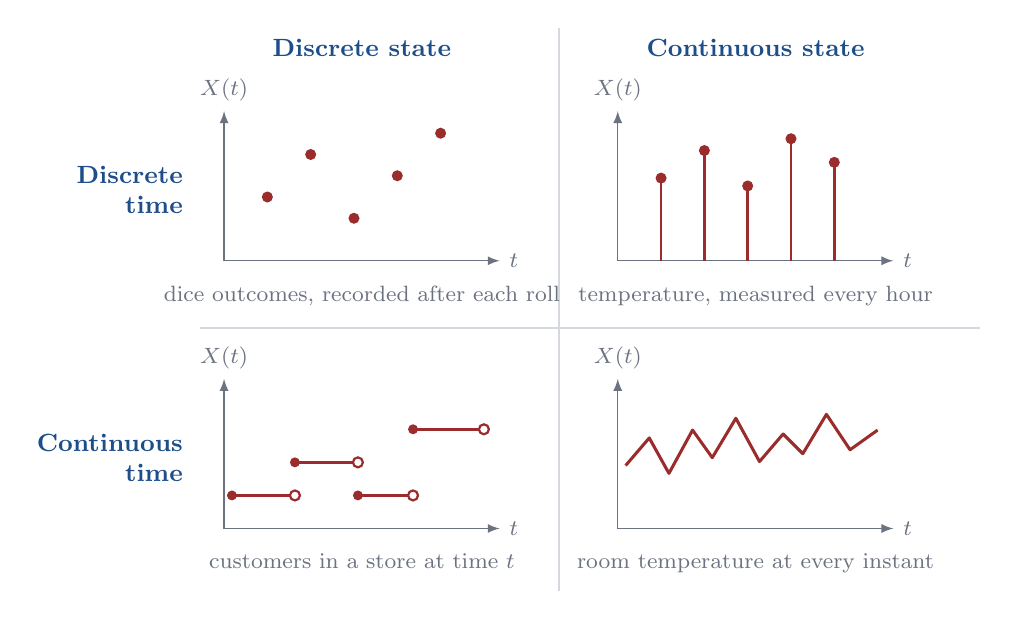
\begin{tikzpicture}[font=\small]
  % Column and row labels, and the rules between the cells.
  \node[font=\small\bfseries, text=accent] at (2.55,7.1) {Discrete state};
  \node[font=\small\bfseries, text=accent] at (7.55,7.1) {Continuous state};
  \node[font=\small\bfseries, text=accent, align=right, anchor=east] at (0.4,5.3) {Discrete\\time};
  \node[font=\small\bfseries, text=accent, align=right, anchor=east] at (0.4,1.9) {Continuous\\time};
  \draw[hair, line width=.6pt] (0.5,3.55) -- (10.4,3.55);
  \draw[hair, line width=.6pt] (5.05,0.2) -- (5.05,7.35);

  % Discrete time, discrete state: dice outcomes, a dot at each roll.
  \panel{0.8}{4.4}{dice outcomes, recorded after each roll}
  \foreach \x/\y in {1/3, 2/5, 3/2, 4/4, 5/6}
    \fill[caution] (0.8+\x*0.55, 4.4+\y*0.27) circle (2pt);

  % Discrete time, continuous state: temperature each hour, a stem per reading.
  \panel{5.8}{4.4}{temperature, measured every hour}
  \foreach \x/\y in {1/1.05, 2/1.40, 3/0.95, 4/1.55, 5/1.25} {
    \draw[caution, line width=.9pt] (5.8+\x*0.55, 4.4) -- ++(0,\y);
    \fill[caution] (5.8+\x*0.55, 4.4+\y) circle (2pt);
  }

  % Continuous time, discrete state: customers in a store, a step function.
  \panel{0.8}{1.0}{customers in a store at time $t$}
  \foreach \a/\b/\y in {0.1/0.9/1, 0.9/1.7/2, 1.7/2.4/1, 2.4/3.3/3} {
    \draw[caution, line width=1.1pt] (0.8+\a, 1.0+\y*0.42) -- (0.8+\b, 1.0+\y*0.42);
    \fill[caution] (0.8+\a, 1.0+\y*0.42) circle (1.8pt);
    \draw[caution, line width=.8pt, fill=white] (0.8+\b, 1.0+\y*0.42) circle (1.8pt);
  }

  % Continuous time, continuous state: room temperature at every instant.
  \panel{5.8}{1.0}{room temperature at every instant}
  \draw[caution, line width=1.1pt, line join=round]
    (5.9,1.8) -- (6.2,2.15) -- (6.45,1.7) -- (6.75,2.25) -- (7.0,1.9) -- (7.3,2.4)
    -- (7.6,1.85) -- (7.9,2.2) -- (8.15,1.95) -- (8.45,2.45) -- (8.75,2.0) -- (9.1,2.25);
\end{tikzpicture}
\end{document}
